% ============================================================
% M3 S2 导学件·波1 臂6 片件 —— 课时12 椭圆的几何性质（2.5.2）＝批C 四片之三（母版照抄制）
% 生成：M3 成卷轮 S2 波1 臂6｜2026-09-14｜编译 cwd＝本目录（中文路径禁 \input 绝对路径）
%   xelatex main-true.tex ×2 → 含详解印本；xelatex main-false.tex ×2 → 纯题版（单源双本）
% 输入链（全只读）：题面库 课时12-2.5.2椭圆的几何性质.md（题面逐字装配）＋ -答案侧.md（值逐字回嵌）
%   ＋ 定稿/批C-课时12-2.5.2椭圆的几何性质.md（详解回嵌源，§9 补产全文区）；toolchain＝qp-m3.sty
%   （钉后版 md5 7c3930362be8a0a2bdf21bbf8ac16573，本地挂载副本，破损即停）。
% 母版体例：详见 成卷/导学件/课时01-坐标法/母版体例说明.md（结构骨架/宏用法/门谱跑法/常见坑）。
% 键账：件内 ansblock 键集 ≡ 题面库片键集 ≡ manifest 键序（21 键，零缺漏零多余）；
%   预习位零键零答案（口令④裁定前口径）；印面号 1—21＝探究 1—16＋课堂评价 17—21，
%   键↔号映射见 值台账-课时12.json。
% 括线判据（承重墙禁放宽）：估高＞8 行（chars/23 栏宽口径）→ 括线模，逐键读数入值台账；
%   其余灰底。本片括线键读数见值台账（门谱实测）。
% 观察注落实（军师令随片下发）：难2＝题面照录在印（多选题型）；简2＝开放题值行
%   「（答案不唯一）」仅详解印本可见（ansblock 纯题档不印，泄答门 false 档零命中）；
%   简6＝档位偏差注（源标0.65→记简档）入件manifest；档位勘误 #19＝0.85（12-简9 无偏差）
%   入件manifest 档位注；逐条读数见 值台账-课时12.json「观察注落实」。
% 字形注：难2 题面「加斯帕尔・蒙日」源 U+30FB 书宋缺字（探针二实证）→印面用「·」(U+00B7)。
% 门谱读数：见过程件 工作区/_tmpM3S2波1臂6_0914/（编译 log、门谱输出、键表）。
% ============================================================
\documentclass[fontset=none]{ctexart}
\usepackage{qp-m3}
% —— 印面逐字符号路由补钉（探针实证 0914：书宋缺 U+2212，▱ 诸字库皆缺→NSC 子块；
%     禁改 sty 本体保 md5；无 ▱/− 用件的片可整块照抄，零副作用） ——
\xeCJKDeclareCharClass{Default}{"2212}%
\setCJKfamilyfont{nscblk}[Path=C:/提示词/工作区/字替对照-0909/variantF/fonts/,BoldFont=NSC-w600.ttf]{NSC-w500.ttf}%
\xeCJKDeclareSubCJKBlock{nscblk}{"25B1}%
\newcommand{\pxparallelogram}{{\CJKfamily{nscblk}▱}}%
% —— 断行微调（纯题档/详解档三零门：CJK 胶收缩 0.01→0.05em；只动伸缩分量不动自然宽度） ——
\xeCJKsetup{CJKglue={\hskip 0.10em plus 0.08em minus 0.05em}}%
% —— 页脚件名（qp-headfoot 复用入口） ——
\renewcommand{\qpzhangming}{第二章\quad 平面解析几何}%
\renewcommand{\qpjianming}{导学件}%

\begin{document}
%装配轮S6三本跨本连续页码（G7方案B）setcounter 注入位
\setcounter{page}{39}

\zhangtitle{第二章\quad 平面解析几何}
\jietitle{2.5.2 椭圆的几何性质}
\mubiaoline
\mubiaomu{1}{掌握椭圆的范围、对称性、顶点、长轴与短轴、离心率等简单几何性质，会用离心率刻画并比较椭圆的扁平程度；}
\mubiaomu{2}{会依条件（长轴、离心率、过点、焦点位置等）求椭圆的标准方程，能判定点与椭圆的位置关系；}
\mubiaomu{3}{能综合运用定义与性质处理焦点三角形、中心弦拼合、距离最值与实际情境问题，会用同焦点椭圆族、蒙日圆等结论求解.}

\vspace{1.7mm}
\begin{multicols}{2}
\emergencystretch=1em

% ============================================================
% 课前预习（知识点导学填空；零键零答案——预习键位按检查口令④裁定前口径，
% \kongbai 空线＋\zhentib 判断题面形，两档等形不泄答）
% ============================================================
\huaxing{课}{前}{预}{习}{知识导学\quad 素养初识}

\zsd{一}{椭圆的简单几何性质}

\tiaomu{1}{范围：\kongbai{}（用\(a\)、\(b\)表示\(x\)、\(y\)的范围）；对称性：椭圆关于\kongbai{}对称；顶点：(±a,0)、(0,±b)；长轴长\kongbai{}、短轴长\kongbai{}；离心率\(e=c/a\)，范围\kongbai{}，\(e\)越大椭圆越\kongbai{}．\zhuzhu{离心率刻画“扁”的程度：\(b/a\)越小（\(e\)越大）越扁；\(a^{2}=b^{2}+c^{2}\)是三个基本量的纽带，与双曲线差号勿混.}}

\zsd{二}{依条件求标准方程·点与椭圆位置}

\tiaomu{1}{待定系数：先定焦点位置设标准形，由条件（长轴、离心率、过点等）列方程组解\(a^{2}\)、\(b^{2}\)；含参方程看\kongbai{}分母定焦点位置．\zhuzhu{点\(P(x_0,y_0)\)与椭圆\(x^{2}/a^{2}+y^{2}/b^{2}=1\)的位置：把坐标代入左端，大于1在外、等于1在上、小于1在内.}}

\zsd{三}{性质与定义的综合应用}

\tiaomu{1}{常用拼合：过焦点的弦与另一侧焦半径凑\(4a\)；中心对称弦与两焦点构成平行四边形；点到直线距离最值可参数化（\(x=a\cos\theta\)、\(y=b\sin\theta\)）或平移切线求．\zhuzhu{同焦点椭圆族：\(a^{2}-b^{2}=c^{2}\)为定值，焦点随大分母在何轴；蒙日圆：椭圆\(x^{2}/a^{2}+y^{2}/b^{2}=1\)的两条互相垂直切线的交点轨迹为\(x^{2}+y^{2}=a^{2}+b^{2}\)（本课时讲解位内容）.}}

\zhenhead{判断正误(正确的打\gou{},错误的打\cha{})}

\zhentib{(1)}{椭圆的离心率\(e\)越小，椭圆越扁．}

\zhentib{(2)}{椭圆\(x^{2}/9+y^{2}/4=1\)关于\(x\)轴、\(y\)轴和原点都对称．}

\zhentib{(3)}{点\(P(x_0,y_0)\)在椭圆\(x^{2}/a^{2}+y^{2}/b^{2}=1\)内部的充要条件是\(x_0^{2}/a^{2}+y_0^{2}/b^{2}<1\)．}

\liubai[9mm]{此处书写}

% ============================================================
% 课中探究（考点探究〔例+变式〕＝练/拓槽 16 键；题后紧跟答案＝ansblock 内嵌，
% 值照答案侧逐字，详解承定稿 §9 回嵌）
% ============================================================
\huaxing{课}{中}{探}{究}{考点探究\quad 素养小结}

% ---------- 探究点一 依条件求方程·点与椭圆位置 ----------
\tjdnr{一}{依条件求方程·点与椭圆位置}{例\textbf{1}}{简单(知识点二)}{设点\(M\)是椭圆\(C\)：\(x^{2}/a^{2}+y^{2}/b^{2}=1\)（\(a>b>0\)）上一动点，椭圆的长轴为\(4\sqrt{3}\)，离心率为\(\sqrt{6}/3\)，求椭圆\(C\)的方程．}
\xiexwei{10mm}

\begin{ansblock}[2章-练-课时12-简1]
% ans:2章-练-课时12-简1
\ansitem{1}{x²/12＋y²/4＝1}
\ansnote{详解}{\(2a=4\sqrt{3}\)，即\(a=2\sqrt{3}\)，\(a^{2}=12\)；\(e=c/a=\sqrt{6}/3\)，即\(c^{2}=(6/9)\times 12=8\)，\(c=2\sqrt{2}\)；\(b^{2}=a^{2}-c^{2}=12-8=4\)．题设已限定焦点在\(x\)轴（方程形如\(x^{2}/a^{2}+y^{2}/b^{2}\)，\(a>b>0\)），故椭圆\(C\)的方程为\(x^{2}/12+y^{2}/4=1\)．}
\end{ansblock}

\liB{变式\textbf{2}}{简单(知识点二)}{}{写出一个焦点在\(x\)轴上，且离心率为\(\sqrt{6}/3\)的椭圆的标准方程：\kongbai{}．}
\xiexwei{12mm}

\begin{ansblock}[2章-练-课时12-简2]
% ans:2章-练-课时12-简2
\ansitem{2}{x²/3＋y²＝1（答案不唯一）}
\ansnote{详解}{设\(x^{2}/a^{2}+y^{2}/b^{2}=1\)（\(a>b>0\)），\(e^{2}=1-b^{2}/a^{2}=6/9=2/3\)，即\(a^{2}=3b^{2}\)．取\(b^{2}=1\)、\(a^{2}=3\)即得\(x^{2}/3+y^{2}=1\)；任取\(b^{2}=t\)（\(t>0\)）、\(a^{2}=3t\)均合题．}
\end{ansblock}

\liB{变式\textbf{3}}{简单(知识点二)}{}{若点\(A(m,1)\)在椭圆\(x^{2}/4+y^{2}/2=1\)的内部，则实数\(m\)的取值范围是\kongbai{}．}
\xiexwei{9mm}

\begin{ansblock}[2章-练-课时12-简3]
% ans:2章-练-课时12-简3
\ansitem{3}{(−√2,√2)}
\ansnote{详解}{点在椭圆内部即代入左端小于1：\(m^{2}/4+1/2<1\)，即\(m^{2}/4<1/2\)，\(m^{2}<2\)，故\(-\sqrt{2}<m<\sqrt{2}\)．}
\end{ansblock}

\liB{变式\textbf{4}}{简单(知识点二)}{}{已知椭圆\(C\)：\(x^{2}/9+y^{2}/b^{2}=1\)（\(b>0\)）上的动点\(P\)到右焦点距离的最小值为\(3-2\sqrt{2}\)，则\(b=\)　　\nobreak(\kongwei)}
\bindopt {\fontsize{10.5pt}{\qpTJgLeadLiti}\selectfont \makebox[\dimexpr0.5\linewidth-1em\relax][l]{A．\(1\)}\makebox[\dimexpr0.5\linewidth-1em\relax][l]{B．\(\sqrt{2}\)}\par}

\bindopt {\fontsize{10.5pt}{\qpTJgLeadLiti}\selectfont \makebox[\dimexpr0.5\linewidth-1em\relax][l]{C．\(\sqrt{3}\)}\makebox[\dimexpr0.5\linewidth-1em\relax][l]{D．\(\sqrt{6}\)}\par}

\begin{ansblock}[2章-练-课时12-简4]
% ans:2章-练-课时12-简4
\ansitem{4}{A}
\ansnote{详解}{\(a^{2}=9\)、\(a=3\)，右焦点\(F_2(c,0)\)．椭圆上点到焦点距离的最小值在长轴（同侧）顶点取得：\(|PF_2|_{\min}=a-c\)．由\(3-c=3-2\sqrt{2}\)得\(c=2\sqrt{2}\)，\(b^{2}=a^{2}-c^{2}=9-8=1\)，\(b=1\)（\(b>0\)）．故选：A．}
\end{ansblock}

\xiaojie{①识别：给长轴/离心率/过点/点位等条件求方程、判定点与椭圆位置关系，判归本题型.}
\bindp {\kaishu ②操作：待定系数设标准形，\(a\)、\(b\)、\(c\)三量两个方程即可定；开放题先写\(a^{2}\)、\(b^{2}\)的约束关系再取特值；点位判定代入左端与1比大小.}
\bindp {\kaishu ③收束：焦点位置由“大分母”或题设限定认准；开放题结论须注明不唯一，并给出通式或两例.}

% ---------- 探究点二 性质与结论的应用 ----------
\tjdnr{二}{性质与结论的应用}{例\textbf{5}}{简单(知识点三)}{若过圆\(x^{2}+y^{2}=8\)上任一点向椭圆\(x^{2}/6+y^{2}/b^{2}=1\)（\(0<b<\sqrt{6}\)）作切线，且两条切线互相垂直，则\(b^{2}=\)　　\nobreak(\kongwei)}
\bindopt {\fontsize{10.5pt}{\qpTJgLeadLiti}\selectfont \makebox[\dimexpr0.5\linewidth-1em\relax][l]{A．\(1\)}\makebox[\dimexpr0.5\linewidth-1em\relax][l]{B．\(3\)}\par}

\bindopt {\fontsize{10.5pt}{\qpTJgLeadLiti}\selectfont \makebox[\dimexpr0.5\linewidth-1em\relax][l]{C．\(2\)}\makebox[\dimexpr0.5\linewidth-1em\relax][l]{D．\(5\)}\par}

\begin{ansblock}[2章-练-课时12-简5]
% ans:2章-练-课时12-简5
\ansitem{5}{C}
\ansnote{详解}{由蒙日圆结论（本课时讲解位2.5.2.20）：\(x^{2}/a^{2}+y^{2}/b^{2}=1\)的两条互相垂直切线的交点轨迹为\(x^{2}+y^{2}=a^{2}+b^{2}\)．题设圆即该椭圆的蒙日圆，故\(6+b^{2}=8\)，\(b^{2}=2\)（满足\(0<b<\sqrt{6}\)）．故选：C．}
\end{ansblock}

\liB{变式\textbf{6}}{简单(知识点三)}{}{已知椭圆\(C\)的方程为\(9x^{2}+4y^{2}=36\)：(1)与椭圆\(C\)有相同焦点的椭圆有多少个？写出其中两个椭圆的方程；(2)与椭圆\(C\)有相同焦点且经过点\((4,\sqrt{5})\)的椭圆有几个？写出符合条件的椭圆方程．}
\xiexwei{12mm}

{\ansblockgrayfalse
\begin{ansblock}[2章-练-课时12-简6]
% ans:2章-练-课时12-简6
\ansitem{6}{(1)无数个，如 x²/3＋y²/8＝1、x²/5＋y²/10＝1（任写两个满足 a²−b²＝5 且焦点在 y 轴者均可）；(2)一个，x²/20＋y²/25＝1}
\ansnote{详解}{\(C\)化标准式\(x^{2}/4+y^{2}/9=1\)，焦点在\(y\)轴，\(c^{2}=9-4=5\)．(1)同焦点即\(a^{2}-b^{2}=5\)且焦点在\(y\)轴，即\(x^{2}/m+y^{2}/(m+5)=1\)（\(m>0\)）对任意\(m>0\)均可，故有无数个；取\(m=3\)、\(m=5\)得\(x^{2}/3+y^{2}/8=1\)、\(x^{2}/5+y^{2}/10=1\)．(2)代入\((4,\sqrt{5})\)：\(16/m+5/(m+5)=1\)，即\(16(m+5)+5m=m(m+5)\)，即\(m^{2}-16m-80=0\)，\((m-20)(m+4)=0\)，\(m=20\)或\(m=-4\)（舍，须\(m>0\)）．故唯一，方程\(x^{2}/20+y^{2}/25=1\)．}
\end{ansblock}}

\liB{变式\textbf{7}}{简单(知识点三)}{}{已知点\(A\)，\(B\)是椭圆\(x^{2}/16+y^{2}/12=1\)上不关于长轴对称的两点，且\(A\)，\(B\)两点到点\(M(m,0)\)的距离相等，求实数\(m\)的取值范围．}
\xiexwei{12mm}

{\ansblockgrayfalse
\begin{ansblock}[2章-练-课时12-简7]
% ans:2章-练-课时12-简7
\ansitem{7}{(−1,1)}
\ansnote{详解}{设\(A(x_1,y_1)\)、\(B(x_2,y_2)\)，“不关于长轴（\(x\)轴）对称”即\(y_1\neq -y_2\)（且\(A\)、\(B\)为不同两点）．\(|AM|=|BM|\)即\((x_1-m)^{2}+y_1^{2}=(x_2-m)^{2}+y_2^{2}\)，即\((x_1-x_2)(x_1+x_2-2m)=y_2^{2}-y_1^{2}\)．椭圆上\(y^{2}=12-(3/4)x^{2}\)，故\(y_2^{2}-y_1^{2}=(3/4)(x_1^{2}-x_2^{2})=(3/4)(x_1-x_2)(x_1+x_2)\)．若\(x_1=x_2\)，则由上式\(y_1^{2}=y_2^{2}\)，结合“不关于长轴对称”得\(y_1=y_2\)，\(A\)、\(B\)重合，矛盾；故\(x_1\neq x_2\)，可约去\((x_1-x_2)\)：\(x_1+x_2-2m=(3/4)(x_1+x_2)\)，即\(2m=(1/4)(x_1+x_2)\)，\(m=(x_1+x_2)/8\)．又\(-4\leqslant x_i\leqslant 4\)且\(x_1\neq x_2\)，故\(-8<x_1+x_2<8\)（两端点\(x_1=x_2=\pm 4\)不能同时取，等号不可达），得\(-1<m<1\)．}
\end{ansblock}}

\liB{变式\textbf{8}}{简单(知识点三)}{}{已知椭圆\(C\)：\(x^{2}/a^{2}+y^{2}/b^{2}=1\)（\(a>b>0\)），四点\(P_1(1,1)\)，\(P_2(0,1)\)，\(P_3(-1,\sqrt{3}/2)\)，\(P_4(1,\sqrt{3}/2)\)中恰有三点在椭圆\(C\)上，求\(C\)的方程．}
\xiexwei{12mm}

{\ansblockgrayfalse
\begin{ansblock}[2章-练-课时12-简8]
% ans:2章-练-课时12-简8
\ansitem{8}{x²/4＋y²＝1}
\ansnote{详解}{\(P_3\)与\(P_4\)关于\(y\)轴对称，而椭圆关于\(y\)轴对称，故\(P_3\)、\(P_4\)同“在”或同“不在”；“恰有三点”须\(P_3\)、\(P_4\)都在其上，第三点为\(P_1\)、\(P_2\)之一．若\(P_1\)在\(C\)上，则与\(P_4\)同横坐标\(x=1\)而纵坐标不同（\(1\neq\sqrt{3}/2\)），同一\(x\)对应椭圆上两点纵坐标互为相反数，矛盾（亦可直接算：\(1/a^{2}+1/b^{2}=1\)与\(1/a^{2}+3/(4b^{2})=1\)相减得\(b=0\)，舍）；故第三点是\(P_2\)．由\(P_2(0,1)\)：\(1/b^{2}=1\)，即\(b^{2}=1\)；由\(P_4(1,\sqrt{3}/2)\)：\(1/a^{2}+3/4=1\)，即\(a^{2}=4\)（\(a>b\)成立）．所以\(C\)：\(x^{2}/4+y^{2}=1\)．回代检验：\(P_1(1,1)\)使\(1/4+1=5/4\neq 1\)，恰不在其上成立．}
\end{ansblock}}

\liB{变式\textbf{9}}{简单(知识点三)}{}{已知椭圆\(C\)：\(x^{2}/4+y^{2}/3=1\)的右焦点为\(F\)，直线\(l\)经过椭圆的右焦点\(F\)，交椭圆\(C\)于\(P\)，\(Q\)两点（点\(P\)在第二象限）．若点\(Q\)关于\(x\)轴的对称点为\(Q'\)，且满足\(PQ\perp FQ'\)，则直线\(l\)的方程是\kongbai{}．}
\xiexwei{12mm}

{\ansblockgrayfalse
\begin{ansblock}[2章-练-课时12-简9]
% ans:2章-练-课时12-简9
\ansitem{9}{x＋y−1＝0}
\ansnote{详解}{\(a^{2}=4\)、\(b^{2}=3\)，即\(c^{2}=1\)，右焦点\(F(1,0)\)．设\(l\)的斜率为\(k\)（\(k\)必存在且\(k\neq 0\)：\(P\)在第二象限、\(F\)在\(x\)轴上），\(l\)：\(y=k(x-1)\)．设\(Q(x_2,y_2)\)，则\(Q'(x_2,-y_2)\)，且\(P\)、\(Q\)、\(F\)共线，故直线\(PQ\)即\(l\)，方向向量\((1,k)\)；向量\(FQ'=(x_2-1,-y_2)=(x_2-1)(1,-k)\)（用\(y_2=k(x_2-1)\)），即\(FQ'\)的方向为\((1,-k)\)（\(x_2\neq 1\)，否则\(Q\)在\(x\)轴上、\(Q\)为顶点使\(P\)不在第二象限，舍）．\(PQ\perp FQ'\)即\((1,k)\cdot(1,-k)=0\)，即\(1-k^{2}=0\)，\(k=\pm 1\)．由\(P\)在第二象限定号：\(k=1\)时\(l\)：\(y=x-1\)与\(x^{2}/4+y^{2}/3=1\)联立得\(7x^{2}-8x-8=0\)，两根之积\(-8/7<0\)，其负根对应\(y=x-1<0\)，点在第三象限，不合；\(k=-1\)时\(l\)：\(y=-(x-1)\)同得\(7x^{2}-8x-8=0\)，负根\(x=(4-6\sqrt{2})/7\)对应\(y=1-x>0\)，点在第二象限成立．故\(k=-1\)，\(l\)：\(y=-(x-1)\)，即\(x+y-1=0\)．}
\end{ansblock}}

\liB{变式\textbf{10}}{简单(知识点三)}{}{天文学家开普勒的行星运动定律可表述为：绕同一中心天体的所有行星的椭圆轨道的半长轴\(a\)的三次方跟它的公转周期\(T\)的二次方的比值都相等，即\(a^{3}/T^{2}=k\)，\(k=GM/4\pi^{2}\)，其中\(M\)为中心天体质量，\(G\)为引力常量。已知地球绕以太阳为中心天体的椭圆轨道的半长轴长约为1.5亿千米，地球的公转周期为1年，距离太阳最远的冥王星绕以太阳为中心天体的椭圆轨道的半长轴长约为60亿千米，取\(\sqrt{10}=3.1\)，则冥王星的公转周期约为　　\nobreak(\kongwei)}
\bindopt {\fontsize{10.5pt}{\qpTJgLeadLiti}\selectfont \makebox[\dimexpr0.5\linewidth-1em\relax][l]{A．157年}\makebox[\dimexpr0.5\linewidth-1em\relax][l]{B．220年}\par}

\bindopt {\fontsize{10.5pt}{\qpTJgLeadLiti}\selectfont \makebox[\dimexpr0.5\linewidth-1em\relax][l]{C．248年}\makebox[\dimexpr0.5\linewidth-1em\relax][l]{D．256年}\par}

\begin{ansblock}[2章-练-课时12-简10]
% ans:2章-练-课时12-简10
\ansitem{10}{C}
\ansnote{详解}{同一中心天体（太阳）即\(a^{3}/T^{2}\)同值，故\(T_2^{2}=(a_2^{3}/a_1^{3})\times T_1^{2}=(60/1.5)^{3}\times 1^{2}=40^{3}=64000\)，\(T_2=\sqrt{64000}=80\sqrt{10}\approx 80\times 3.1=248\)（年）．故选：C．}
\end{ansblock}

\xiaojie{①识别：用蒙日圆、同焦点族、对称性、开普勒定律等性质与结论求解的问题，判归本题型.}
\bindp {\kaishu ②操作：先辨认性质结论（蒙日圆\(x^{2}+y^{2}=a^{2}+b^{2}\)、同焦点族\(a^{2}-b^{2}\)定值、中心对称拼合\(4a\)），把几何条件翻译成\(a\)、\(b\)、\(c\)的方程；对称等距问题设坐标代入距离公式约去公因式.}
\bindp {\kaishu ③收束：约分前先证公因式非零（反设重合导矛盾）；定号条件（象限、范围）最后回验一遍，两端开闭看等号能否取到.}

% ---------- 探究点三 综合拼合与最值 ----------
\tjdnr{三}{综合拼合与最值}{例\textbf{11}}{中档(知识点三)}{\(AB\)是平面上长度为4的一条线段，\(P\)是平面上一个动点，且\(|PA|+|PB|=6\)，\(M\)是\(AB\)的中点，则\(|PM|\)的取值范围是\kongbai{}．}
\xiexwei{12mm}

{\ansblockgrayfalse
\begin{ansblock}[2章-练-课时12-中1]
% ans:2章-练-课时12-中1
\ansitem{11}{[√5,3]}
\ansnote{详解}{\(|PA|+|PB|=6>|AB|=4\)，故\(P\)的轨迹是以\(A\)、\(B\)为焦点、\(2a=6\)的椭圆．以\(M\)为原点、\(AB\)所在直线为\(x\)轴建系，则\(A(-2,0)\)、\(B(2,0)\)，\(c=2\)、\(a=3\)、\(b^{2}=a^{2}-c^{2}=9-4=5\)，轨迹\(x^{2}/9+y^{2}/5=1\)．\(M\)即椭圆中心，\(|PM|\)为中心到椭圆上点的距离：\(|PM|^{2}=x^{2}+y^{2}=x^{2}+5(1-x^{2}/9)=5+(4/9)x^{2}\)，\(x^{2}\in[0,9]\)，故\(|PM|^{2}\in[5,9]\)，\(|PM|\in[\sqrt{5},3]\)（最小在短轴端点\(=b\)，最大在长轴端点\(=a\)）．}
\end{ansblock}}

\liB{变式\textbf{12}}{中档(知识点三)}{}{设椭圆\(C\)：\(x^{2}/4+y^{2}/3=1\)的右焦点为\(F\)，过原点\(O\)的动直线\(l\)与椭圆\(C\)交于\(A\)，\(B\)两点，那么\(\triangle ABF\)的周长的取值范围为\kongbai{}．}
\xiexwei{12mm}

{\ansblockgrayfalse
\begin{ansblock}[2章-练-课时12-中2]
% ans:2章-练-课时12-中2
\ansitem{12}{[4＋2√3, 8)}
\ansnote{详解}{\(a=2\)、\(b=\sqrt{3}\)、\(c=1\)，右焦点\(F(1,0)\)，记左焦点\(F_1(-1,0)\)．\(l\)过原点，\(A\)、\(B\)关于中心\(O\)对称，故\(O\)是\(AB\)的中点，又\(O\)是\(FF_1\)的中点，所以四边形\(AFBF_1\)是平行四边形，\(|BF|=|AF_1|\)．周长\(L=|AB|+|AF|+|BF|=|AB|+(|AF|+|AF_1|)=|AB|+2a=|AB|+4\)．求\(|AB|\)：\(l\)的斜率不为0（斜率为0时\(A\)、\(B\)为长轴端点，与\(F\)共线，三角形退化），设\(l\)：\(x=my\)，代入得\(y^{2}=12/(3m^{2}+4)\)，\(|AB|=2\sqrt{x^{2}+y^{2}}=2\sqrt{(m^{2}+1)y^{2}}=2\sqrt{12(m^{2}+1)/(3m^{2}+4)}=4\sqrt{1-1/(3m^{2}+4)}\)．\(m^{2}\geqslant 0\)，即\(3m^{2}+4\geqslant 4\)，\(1-1/(3m^{2}+4)\in[3/4,1)\)，故\(|AB|\in[2\sqrt{3},4)\)．所以\(L=|AB|+4\in[4+2\sqrt{3},8)\)（上端\(|AB|\to 2a=4\)对应直线趋于长轴、三角形退化，取开）．}
\end{ansblock}}

\liB{变式\textbf{13}}{中档(知识点三)}{}{点\(P\)在椭圆\(x^{2}/16+y^{2}/9=1\)上，点\(P\)到直线\(3x-4y=24\)的最大距离和最小距离为\kongbai{}．}
\xiexwei{12mm}

{\ansblockgrayfalse
\begin{ansblock}[2章-练-课时12-中3]
% ans:2章-练-课时12-中3
\ansitem{13}{最大 12(2＋√2)/5，最小 12(2−√2)/5}
\ansnote{详解}{设\(P(4\cos\theta,3\sin\theta)\)，则\(d=|3\cdot 4\cos\theta-4\cdot 3\sin\theta-24|/\sqrt{3^{2}+4^{2}}=|12\cos\theta-12\sin\theta-24|/5=|12\sqrt{2}\cos(\theta+\pi/4)-24|/5\)．因\(12\sqrt{2}<24\)，\(\cos(\theta+\pi/4)\in[-1,1]\)时\(12\sqrt{2}\cos(\theta+\pi/4)-24\)恒为负，绝对值直接翻号：\(d=(24-12\sqrt{2}\cos(\theta+\pi/4))/5\)．\(\cos(\theta+\pi/4)=-1\)时\(d_{\max}=(24+12\sqrt{2})/5=12(2+\sqrt{2})/5\)；\(\cos(\theta+\pi/4)=1\)时\(d_{\min}=(24-12\sqrt{2})/5=12(2-\sqrt{2})/5\)．（另法：设与\(3x-4y=24\)平行的切线\(3x-4y=t\)，由判别式为0得\(t=\pm 12\sqrt{2}\)，两切线到已知直线的距离\(|24\mp 12\sqrt{2}|/5\)即最小、最大值，结果一致．）}
\end{ansblock}}

\liB{变式\textbf{14}}{中档(知识点三)}{}{在大西北的荒漠上，\(A\)，\(B\)两地相距 2 km，正准备在荒漠上围成一片以\(AB\)为一条对角线的平行四边形区域，建立农艺园．按照规划，围墙总长度为 8 km．(1)农艺园的最大面积能达到多少?(2)该荒漠上有一条直线型水沟刚好过点\(A\)，且与\(AB\)成 45°角，现要对整条水沟进行加固改造，但考虑到今后农艺园内的水沟要重新设计改造，因此该水沟被农艺园围住的部分暂不加固，那么暂不加固的部分有多长?}
\xiexwei{12mm}

{\ansblockgrayfalse
\begin{ansblock}[2章-练-课时12-中4]
% ans:2章-练-课时12-中4
\ansitem{14}{(1)2√3 km²；(2)24/7 km}
\ansnote{详解}{设平行四边形为\(ADBC\)（\(AB\)、\(CD\)为两条对角线），周长8 km即相邻两边之和\(|CA|+|CB|=4\) km，故另两顶点\(C\)（及\(D\)）在以\(A\)、\(B\)为焦点的椭圆上：\(2a=4\)、\(2c=|AB|=2\)，\(a=2\)、\(c=1\)、\(b^{2}=3\)．以\(AB\)所在直线为\(x\)轴、\(AB\)中点为原点建系，\(A(-1,0)\)、\(B(1,0)\)，椭圆\(x^{2}/4+y^{2}/3=1\)（\(y\neq 0\)，退化时不成四边形）．(1)平行四边形\(ADBC\)的面积\(=2S_{\triangle ABC}=2\times(1/2\times|AB|\times|y_C|)=2|y_C|\)，而\(C\)在椭圆上即\(|y_C|\leqslant b=\sqrt{3}\)，当\(C\)为短轴端点时取等，故最大面积\(=2\sqrt{3}\) km\(^{2}\)．(2)水沟过\(A(-1,0)\)且与\(AB\)（\(x\)轴）成45°角，取斜率1，方程\(y=x+1\)（取斜率\(-1\)时由对称性弦长相同）．“被农艺园围住的部分”即直线被椭圆截得的弦（口径已由亲算⑥注记2钉死，非“最大面积菱形”口径）：代入\(x^{2}/4+(x+1)^{2}/3=1\)，即\(3x^{2}+4(x^{2}+2x+1)=12\)，即\(7x^{2}+8x-8=0\)，\(x_1+x_2=-8/7\)，\(x_1x_2=-8/7\)，\(|x_1-x_2|=\sqrt{(8/7)^{2}+4\times 8/7}=\sqrt{288/49}=(12\sqrt{2})/7\)，弦长\(=\sqrt{1+k^{2}}\,|x_1-x_2|=\sqrt{2}\times(12\sqrt{2})/7=24/7\) km．}
\end{ansblock}}

\xiaojie{①识别：定义轨迹＋范围、中心弦周长、参数法距离最值、实际情境建模式综合题，判归本题型.}
\bindp {\kaishu ②操作：先把几何情境翻译成椭圆（定义三查：定值、定值大于焦距、剔退化），再选工具——中心对称拼\(2a\)、参数化或平移切线求最值、设\(x=my\)避斜率讨论.}
\bindp {\kaishu ③收束：范围题开闭端逐一交代（退化位取开、可取位取闭）；实际题答数带单位，模型前提（不退化、不共线）在文首声明.}

% ---------- 探究点四 压轴构形 ----------
\tjdnr{四}{压轴构形}{例\textbf{15}}{难(知识点三)}{椭圆\(C\)：\(x^{2}/18+y^{2}/b^{2}=1\)的上、下顶点分别为\(A\)，\(C\)，如图，点\(B\)在椭圆上，平面四边形\(ABCD\)满足\(\angle BAD=\angle BCD=90^{\circ}\)，且\(S_{\triangle ABC}=2S_{\triangle ADC}\)，则该椭圆的短轴长为\kongbai{}．}
\ansfig{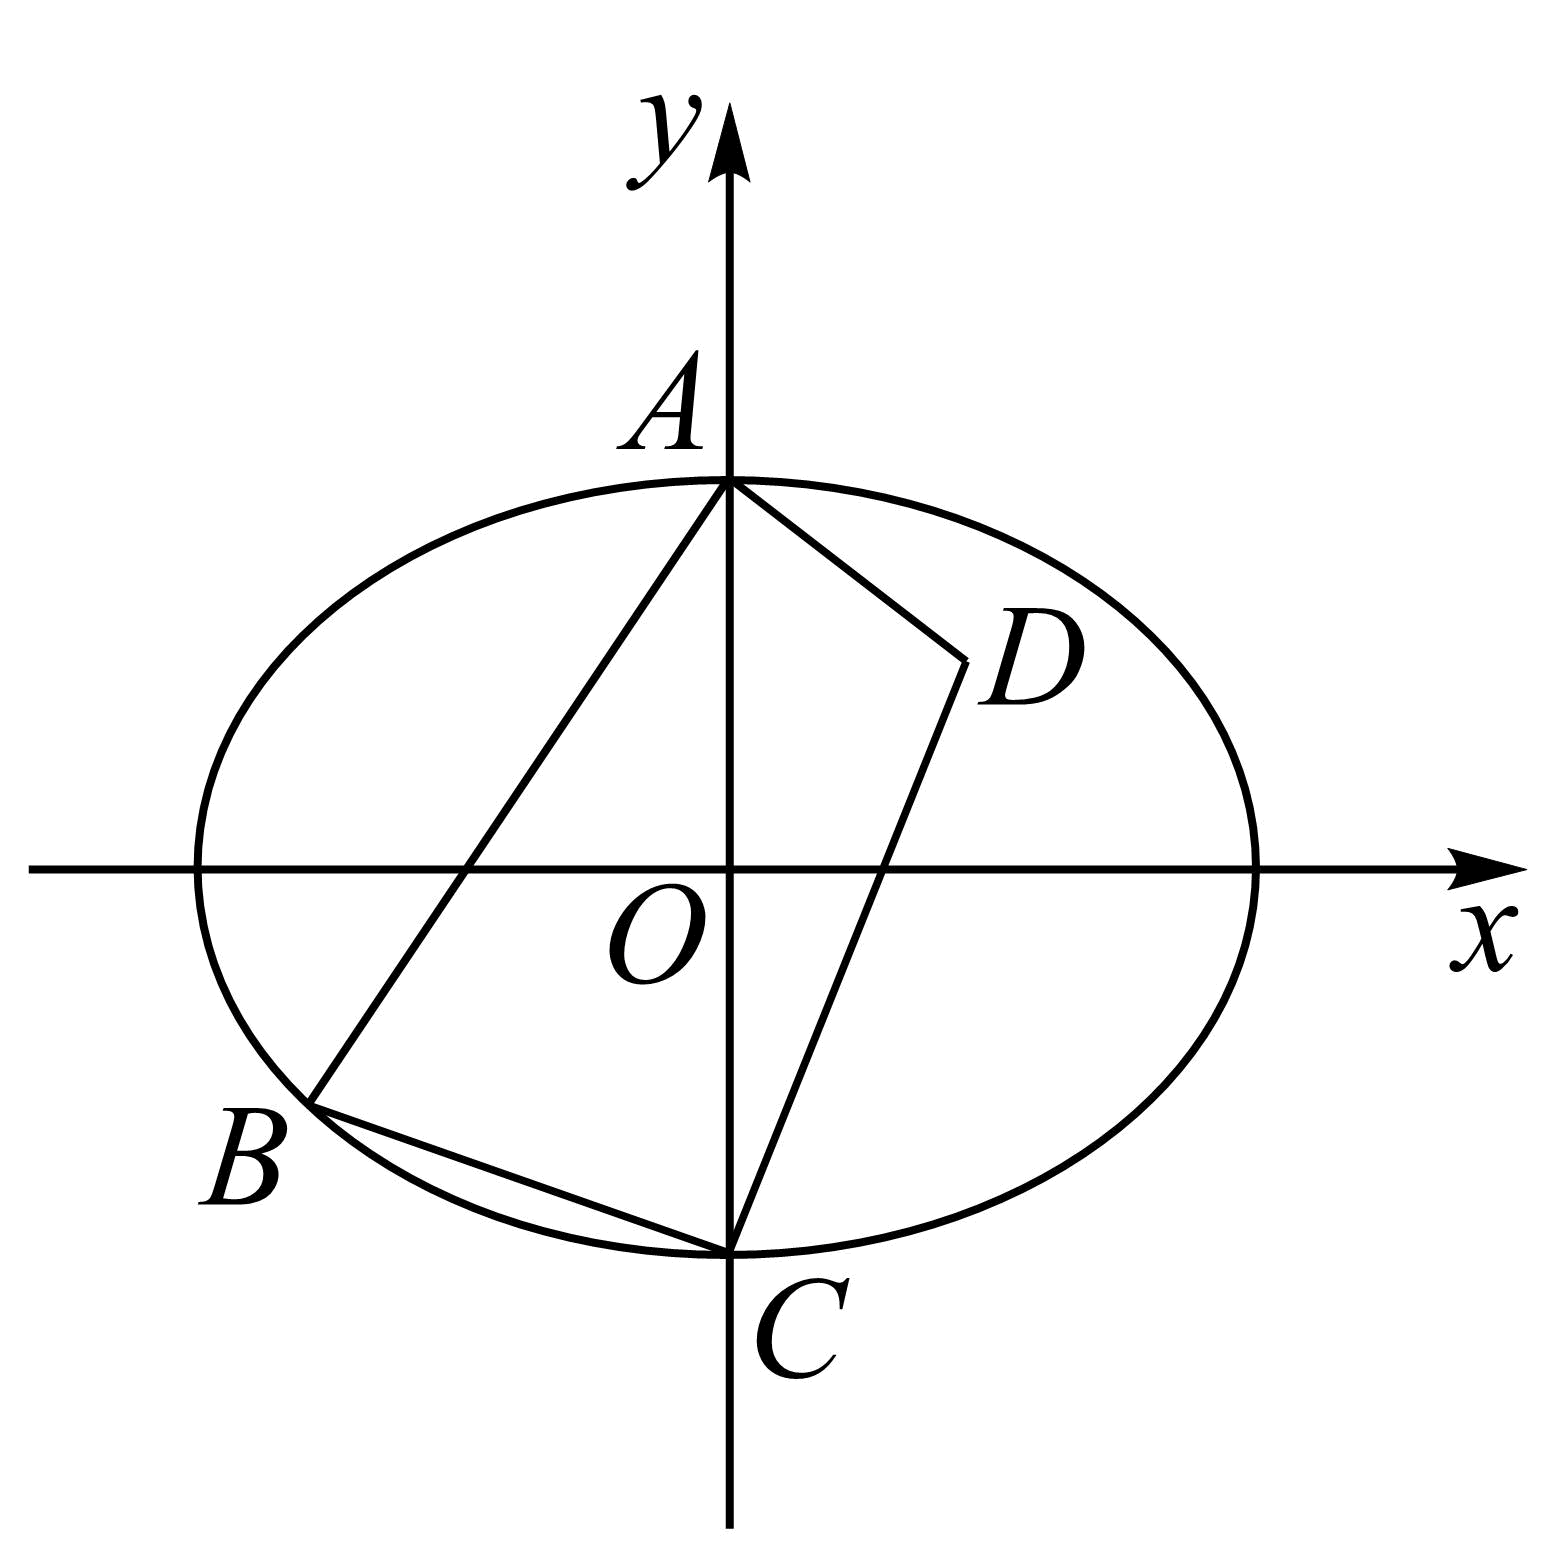
\includegraphics[width=42mm]{figs/12-难1.png}}
\xiexwei{12mm}

{\ansblockgrayfalse
\begin{ansblock}[2章-练-课时12-难1]
% ans:2章-练-课时12-难1
\ansitem{15}{6}
\ansnote{详解}{\(A(0,b)\)、\(C(0,-b)\)，设\(B(x_1,y_1)\)、\(D(x_2,y_2)\)．\(\angle BAD=\angle BCD=90^{\circ}\)即\(A\)、\(C\)都在以\(BD\)为直径的圆上，即\(A\)、\(B\)、\(C\)、\(D\)四点共圆，圆心为\(BD\)的中点\(((x_1+x_2)/2,(y_1+y_2)/2)\)．又该圆过\(A\)、\(C\)，圆心在弦\(AC\)的垂直平分线（即\(x\)轴）上，故\((y_1+y_2)/2=0\)，即\(y_2=-y_1\)．面积条件：\(\triangle ABC\)与\(\triangle ADC\)共底\(AC\)（在\(y\)轴上），故\(S_{\triangle ABC}/S_{\triangle ADC}=|x_1|/|x_2|=2\)，即\(|x_1|=2|x_2|\)；因\(B\)、\(D\)分居\(y\)轴两侧，取\(x_1=-2x_2\)．于是圆心为\((x_1/4,0)\)，半径平方\(R^{2}=(x_1-x_1/4)^{2}+y_1^{2}=(9/16)x_1^{2}+y_1^{2}\)．把\(A(0,b)\)代入圆方程：\((x_1/4)^{2}+b^{2}=(9/16)x_1^{2}+y_1^{2}\)，即\(b^{2}=(1/2)x_1^{2}+y_1^{2}\)……①又\(B\)在椭圆上：\(x_1^{2}/18+y_1^{2}/b^{2}=1\)，配合①消\(x_1\)（\(x_1^{2}=2(b^{2}-y_1^{2})\)）：\((b^{2}-y_1^{2})/9+y_1^{2}/b^{2}=1\)，乘\(9b^{2}\)得\(b^{4}-b^{2}y_1^{2}+9y_1^{2}-9b^{2}=0\)，即\((b^{2}-9)(b^{2}-y_1^{2})=0\)．\(B\)异于上、下顶点，故\(y_1^{2}<b^{2}\)，\(b^{2}-y_1^{2}\neq 0\)，只能\(b^{2}=9\)，\(b=3\)，短轴长\(2b=6\)．（存在性核验：\(b^{2}=9\)时①化为\(x_1^{2}=18-2y_1^{2}\)，与椭圆\(x^{2}/18+y^{2}/9=1\)同解，构型可行．取\(y_1=0\)：\(B(3\sqrt{2},0)\)、\(D(-3\sqrt{2}/2,0)\)、\(A(0,3)\)、\(C(0,-3)\)，\(AB\cdot AD=(3\sqrt{2},-3)\cdot(-3\sqrt{2}/2,-3)=-9+9=0\)成立，\(\angle BAD=90^{\circ}\)，同理\(\angle BCD=90^{\circ}\)；\(S_{\triangle ABC}=1/2\times 6\times 3\sqrt{2}=9\sqrt{2}\)、\(S_{\triangle ADC}=1/2\times 6\times(3\sqrt{2}/2)=9\sqrt{2}/2\)，比值2成立．）}
\end{ansblock}}

\liB{变式\textbf{16}}{难(知识点三)}{\duoxuan\hspace{0.6em}}{画法几何的创始人——法国数学家加斯帕尔·蒙日发现：与椭圆相切的两条垂直切线的交点的轨迹是以椭圆中心为圆心的圆，我们通常称这个圆为蒙日圆．已知椭圆\(C\)：\(x^{2}/a^{2}+y^{2}/b^{2}=1\)（\(a>b>0\)）的离心率为\(\sqrt{2}/2\)，\(F_1\)，\(F_2\)分别为椭圆的左、右焦点，\(A\)，\(B\)为椭圆上两个动点，直线\(l\)的方程为\(bx+ay-a^{2}-b^{2}=0\)，下列说法正确的是\nobreak(\kongwei)}

\lxopt{A．\(C\)的蒙日圆的方程为\(x^{2}+y^{2}=3b^{2}\)}

\lxopt{B．对直线\(l\)上任意一点\(P\)，\(PA\cdot PB>0\)}

\lxopt{C．过点\(A\)作\(l\)的垂线，垂足为\(H\)，则\(|AH|-|AF_2|\)的最小值为\((4\sqrt{3}/3)b\)}

\lxopt{D．若矩形\(MNGH\)的四条边均与\(C\)相切，则矩形\(MNGH\)面积的最大值为\(6b^{2}\)}

{\ansblockgrayfalse
\begin{ansblock}[2章-练-课时12-难2]
% ans:2章-练-课时12-难2
\ansitem{16}{AD}
\ansnote{详解}{\(e=\sqrt{2}/2\)，即\(c^{2}/a^{2}=1/2\)，\(a^{2}=2b^{2}\)，\(c^{2}=a^{2}-b^{2}=b^{2}\)，即\(a=\sqrt{2}b\)、\(c=b\)．A：蒙日圆半径平方\(r^{2}=a^{2}+b^{2}=3b^{2}\)，圆心为中心，故\(x^{2}+y^{2}=3b^{2}\)，正确．B：把\(P(b,a)\)代入\(l\)：\(b\cdot b+a\cdot a-a^{2}-b^{2}=0\)，故\(P(b,a)\)在\(l\)上；又\(b^{2}+a^{2}=a^{2}+b^{2}=r^{2}\)，故\(P\)在蒙日圆上，过\(P\)的两条切线互相垂直，取\(A\)、\(B\)为两切点时\(PA\cdot PB=0\)，“任意一点恒有\(PA\cdot PB>0\)”不成立，错误．C：\(|AF_1|+|AF_2|=2a\)，故\(|AH|-|AF_2|=|AH|+|AF_1|-2a\geqslant d(F_1,l)-2a\)．\(d(F_1,l)=|b\cdot(-c)+a\cdot 0-a^{2}-b^{2}|/\sqrt{a^{2}+b^{2}}=(bc+a^{2}+b^{2})/\sqrt{a^{2}+b^{2}}=(b^{2}+2b^{2}+b^{2})/(\sqrt{3}b)=4b/\sqrt{3}=(4\sqrt{3}/3)b\)．故\(|AH|-|AF_2|\)的最小值为\((4\sqrt{3}/3)b-2a=(4\sqrt{3}/3)b-2\sqrt{2}b\)，并非\((4\sqrt{3}/3)b\)，错误（\((4\sqrt{3}/3)b\)只是\(F_1\)到\(l\)的距离，漏减\(2a\)）．D：矩形四边均与\(C\)相切，则相邻两边为一对互相垂直的切线，其四个顶点都在蒙日圆上，即蒙日圆是矩形的外接圆，对角线为直径\(2r=2\sqrt{3}b\)．设两邻边为\(p\)、\(q\)，则\(p^{2}+q^{2}=(2r)^{2}=12b^{2}\)，面积\(pq\leqslant(p^{2}+q^{2})/2=6b^{2}\)，当\(p=q=\sqrt{6}b\)（正方形、对角线落在坐标轴上）时取等，正确．故选：AD．}
\end{ansblock}}

\xiaojie{①识别：四点共圆、蒙日圆综合、切线构形等压轴题，判归本题型.}
\bindp {\kaishu ②操作：直角转直径圆（圆周角定理逆用）先证共圆；蒙日圆题先化简\(a\)、\(b\)、\(c\)关系再逐项核对；切线矩形用外接圆直径＋均值不等式.}
\bindp {\kaishu ③收束：多选题逐项独立判定、反例一举即错；存在性核验（构型可取）随题载明防假解.}

% ============================================================
% 课堂评价 G5（恒5＝3单选+2填空＝导槽 G1~G5；ketang 新制顺排可跨栏，禁 \vbox 装栏）
% 印面号 17—21；多选门：本片正文多选 1（难2）≤4 合规
% ============================================================
\begin{ketang}{本组共5题（第17—21题），17—19为单选，20—21为填空．}

\jiancestem{{\fontsize{11.4pt}{14pt}\selectfont\heihao {\numboldjian 17}．}\hspace{4.1mm}\tieside{简单(知识点一)}\hspace{2.2mm}下列四个椭圆中，形状最扁的是\nobreak(\kongwei)}

\bindopt {\fontsize{10.5pt}{\qpTJgLeadPingjia}\selectfont \makebox[\dimexpr0.5\linewidth-1em\relax][l]{A．\(x^{2}/20+y^{2}/9=1\)}\makebox[\dimexpr0.5\linewidth-1em\relax][l]{B．\(x^{2}/20+y^{2}/10=1\)}\par}

\bindopt {\fontsize{10.5pt}{\qpTJgLeadPingjia}\selectfont \makebox[\dimexpr0.5\linewidth-1em\relax][l]{C．\(x^{2}/20+y^{2}/11=1\)}\makebox[\dimexpr0.5\linewidth-1em\relax][l]{D．\(x^{2}/20+y^{2}/12=1\)}\par}

\begin{ansblock}[2章-导-课时12-G1]
% ans:2章-导-课时12-G1
\ansitem{17}{A}
\ansnote{详解}{\(e=\sqrt{1-b^{2}/a^{2}}\)，四个椭圆\(a^{2}\)同为20，故\(b^{2}\)越小\(e\)越大、椭圆越扁．\(b^{2}/a^{2}\)依次为\(9/20<10/20<11/20<12/20\)，所以\(x^{2}/20+y^{2}/9=1\)的离心率最大，形状最扁．故选：A．}
\end{ansblock}

\jiancestem{{\fontsize{11.4pt}{14pt}\selectfont\heihao {\numboldjian 18}．}\hspace{4.1mm}\tieside{简单(知识点三)}\hspace{2.2mm}已知两定点\(A(-2,0)\)和\(B(2,0)\)，动点\(P(x,y)\)在直线\(l\)：\(y=x+4\)上移动，椭圆\(C\)以\(A\)，\(B\)为焦点且经过点\(P\)，则椭圆\(C\)的离心率的最大值为\nobreak(\kongwei)}

\bindopt {\fontsize{10.5pt}{\qpTJgLeadPingjia}\selectfont \makebox[\dimexpr0.5\linewidth-1em\relax][l]{A．\(\sqrt{10}/10\)}\makebox[\dimexpr0.5\linewidth-1em\relax][l]{B．\(\sqrt{10}/5\)}\par}

\bindopt {\fontsize{10.5pt}{\qpTJgLeadPingjia}\selectfont \makebox[\dimexpr0.5\linewidth-1em\relax][l]{C．\(\sqrt{5}/5\)}\makebox[\dimexpr0.5\linewidth-1em\relax][l]{D．\(2\sqrt{5}/5\)}\par}

{\ansblockgrayfalse
\begin{ansblock}[2章-导-课时12-G2]
% ans:2章-导-课时12-G2
\ansitem{18}{B}
\ansnote{详解}{\(2c=|AB|=4\)，\(c=2\)；\(2a=|PA|+|PB|\)，\(e=c/a\)最大即\(a\)最小，即\(|PA|+|PB|\)最小．求折线和最小：\(A\)关于\(l\)：\(x-y+4=0\)的对称点\(A'(x',y')\)，由公式\(x'=x_0-2\cdot(x_0-y_0+4)/2=-2-2=-4\)，\(y'=y_0+2\cdot(x_0-y_0+4)/2=0+2=2\)，即\(A'(-4,2)\)（与“\(AA'\perp l\)、\(AA'\)中点在\(l\)上”两条件验算一致）．于是\(|PA|+|PB|=|PA'|+|PB|\geqslant|A'B|=\sqrt{(-4-2)^{2}+2^{2}}=\sqrt{40}=2\sqrt{10}\)，当\(P\)为\(A'B\)与\(l\)的交点时取等．故\(2a\geqslant 2\sqrt{10}\)，\(a\geqslant\sqrt{10}\)，\(e=c/a\leqslant 2/\sqrt{10}=\sqrt{10}/5\)．故选：B．}
\end{ansblock}}

\jiancestem{{\fontsize{11.4pt}{14pt}\selectfont\heihao {\numboldjian 19}．}\hspace{4.1mm}\tieside{简单(知识点三)}\hspace{2.2mm}已知椭圆\(C\)：\(x^{2}/a^{2}+y^{2}/b^{2}=1\)（\(a>b>0\)）的离心率为\(\sqrt{6}/3\)，直线\(ax-by=0\)与圆\(M\)：\(x^{2}+y^{2}-mx+1/4=0\)相切，则实数\(m\)的值是\nobreak(\kongwei)}

\bindopt {\fontsize{10.5pt}{\qpTJgLeadPingjia}\selectfont \makebox[\dimexpr0.5\linewidth-1em\relax][l]{A．\(\pm 1\)}\makebox[\dimexpr0.5\linewidth-1em\relax][l]{B．\(\pm 2\)}\par}

\bindopt {\fontsize{10.5pt}{\qpTJgLeadPingjia}\selectfont \makebox[\dimexpr0.5\linewidth-1em\relax][l]{C．\(\pm 4\)}\makebox[\dimexpr0.5\linewidth-1em\relax][l]{D．\(\pm 8\)}\par}

{\ansblockgrayfalse
\begin{ansblock}[2章-导-课时12-G3]
% ans:2章-导-课时12-G3
\ansitem{19}{B}
\ansnote{详解}{\(e=\sqrt{6}/3\)，即\(c^{2}/a^{2}=2/3\)，\(b^{2}/a^{2}=1/3\)，\(a=\sqrt{3}b\)，直线\(ax-by=0\)即\(y=(a/b)x=\sqrt{3}x\)．圆\(M\)化为\((x-m/2)^{2}+y^{2}=(m^{2}-1)/4\)，圆心\((m/2,0)\)、半径\(r=\frac{1}{2}\sqrt{m^{2}-1}\)（须\(m^{2}>1\)）．相切即圆心到直线\(\sqrt{3}x-y=0\)的距离等于半径：\(|\sqrt{3}\cdot m/2|/2=\frac{1}{2}\sqrt{m^{2}-1}\)，平方得\(3m^{2}/16=(m^{2}-1)/4\)，即\(3m^{2}=4m^{2}-4\)，\(m^{2}=4\)，\(m=\pm 2\)（满足\(m^{2}>1\)）．故选：B．}
\end{ansblock}}

\jiancestem{{\fontsize{11.4pt}{14pt}\selectfont\heihao {\numboldjian 20}．}\hspace{4.1mm}\tieside{简单(知识点一)}\hspace{2.2mm}椭圆\(x^{2}/5+y^{2}/m=1\)的焦点坐标是\kongbai{}．}
\xiexwei{10mm}

\begin{ansblock}[2章-导-课时12-G4]
% ans:2章-导-课时12-G4
\ansitem{20}{(±√(5−m),0)（0＜m＜5）；(0,±√(m−5))（m＞5）}
\ansnote{详解}{须\(m>0\)且\(m\neq 5\)．当\(0<m<5\)时焦点在\(x\)轴，\(a^{2}=5\)、\(b^{2}=m\)，\(c^{2}=5-m\)，焦点为\((\pm\sqrt{5-m},0)\)；当\(m>5\)时焦点在\(y\)轴，\(a^{2}=m\)、\(b^{2}=5\)，\(c^{2}=m-5\)，焦点为\((0,\pm\sqrt{m-5})\)．}
\end{ansblock}

\jiancestem{{\fontsize{11.4pt}{14pt}\selectfont\heihao {\numboldjian 21}．}\hspace{4.1mm}\tieside{简单(知识点一)}\hspace{2.2mm}根据下列条件，求椭圆的离心率：(1)长轴与短轴之比为 3∶2；(2)以短轴的两个端点和一个焦点为顶点的三角形是等边三角形．}
\xiexwei{12mm}

\begin{ansblock}[2章-导-课时12-G5]
% ans:2章-导-课时12-G5
\ansitem{21}{(1)√5/3；(2)√3/2}
\ansnote{详解}{(1)\(a:b=3:2\)，取\(a=3k\)、\(b=2k\)，\(c^{2}=a^{2}-b^{2}=5k^{2}\)，\(e=c/a=\sqrt{5}k/3k=\sqrt{5}/3\)．(2)短轴端点\((0,\pm b)\)与焦点\((c,0)\)构成等边三角形：底边\(2b\)，腰\(\sqrt{b^{2}+c^{2}}=a\)，故\(a=2b\)；\(c^{2}=a^{2}-b^{2}=3b^{2}\)，\(e=c/a=\sqrt{3}b/2b=\sqrt{3}/2\)．}
\end{ansblock}

\end{ketang}

% ---- 尾块（\tailfill 置 \end{multicols} 前；无参＝内容尾随框，件侧不擅自定高） ----
\tailfill

\end{multicols}
\end{document}
